\chapter{Manuais de usuario}

%Incluirán toda a información precisa para aquelas persoas que utilicen o Sistema: instalación, utilización, configuración,
%mensaxes de erro, etc. A documentación do usuario debe ser autocontida, é dicir, para o seu entendemento o usuario final
%non debe precisar da lectura doutro manual técnico.
O manual de usuario proporciona a información necesaria para o usuario final que desexa empregar o sistema de forma autónoma; é dicir, que o usuario non precise ler outro manual para empregar a
aplicación.

Para acceder á aplicación, o usuario debe acceder á seguinte URL: \url{http://13.53.65.240:8080/TROPOMIVisor/} , podendo ver a interface da figura \ref{fig:interfaz}. Nela, preséntaselle un
desplegable para elixir o parámetro, entre os 4 que hai dispoñibles (CO, SO2, NO2 ou O3); e un calendario dende o que pode elixir o mes do que quere consultar os datos. Ó realizar un cambio en
calquera destes dous parámetros, actualizarase automaticamente o mapa, amosándose o gráfico correspondente. O usuario deberá ter en conta o rango de datas dispoñible para consultar os datos, que
neste traballo é a partir de xaneiro de 2023. Ademais, deberá ter en conta que os datos do mes anterior (por exemplo, de xaneiro de 2024) non estarán dispoñibles ata aproximadamente o día 11 do
seguinte mes (neste caso, o 11 de febreiro), debido á latencia á hora de procesar os datos tanto no servidor local como por parte de COPERNICUS. Se intenta visualizar o mapa para un mes no que non
hai datos, a imaxe mostrará unha mensaxe de erro.

\begin{figure}
    \centerline{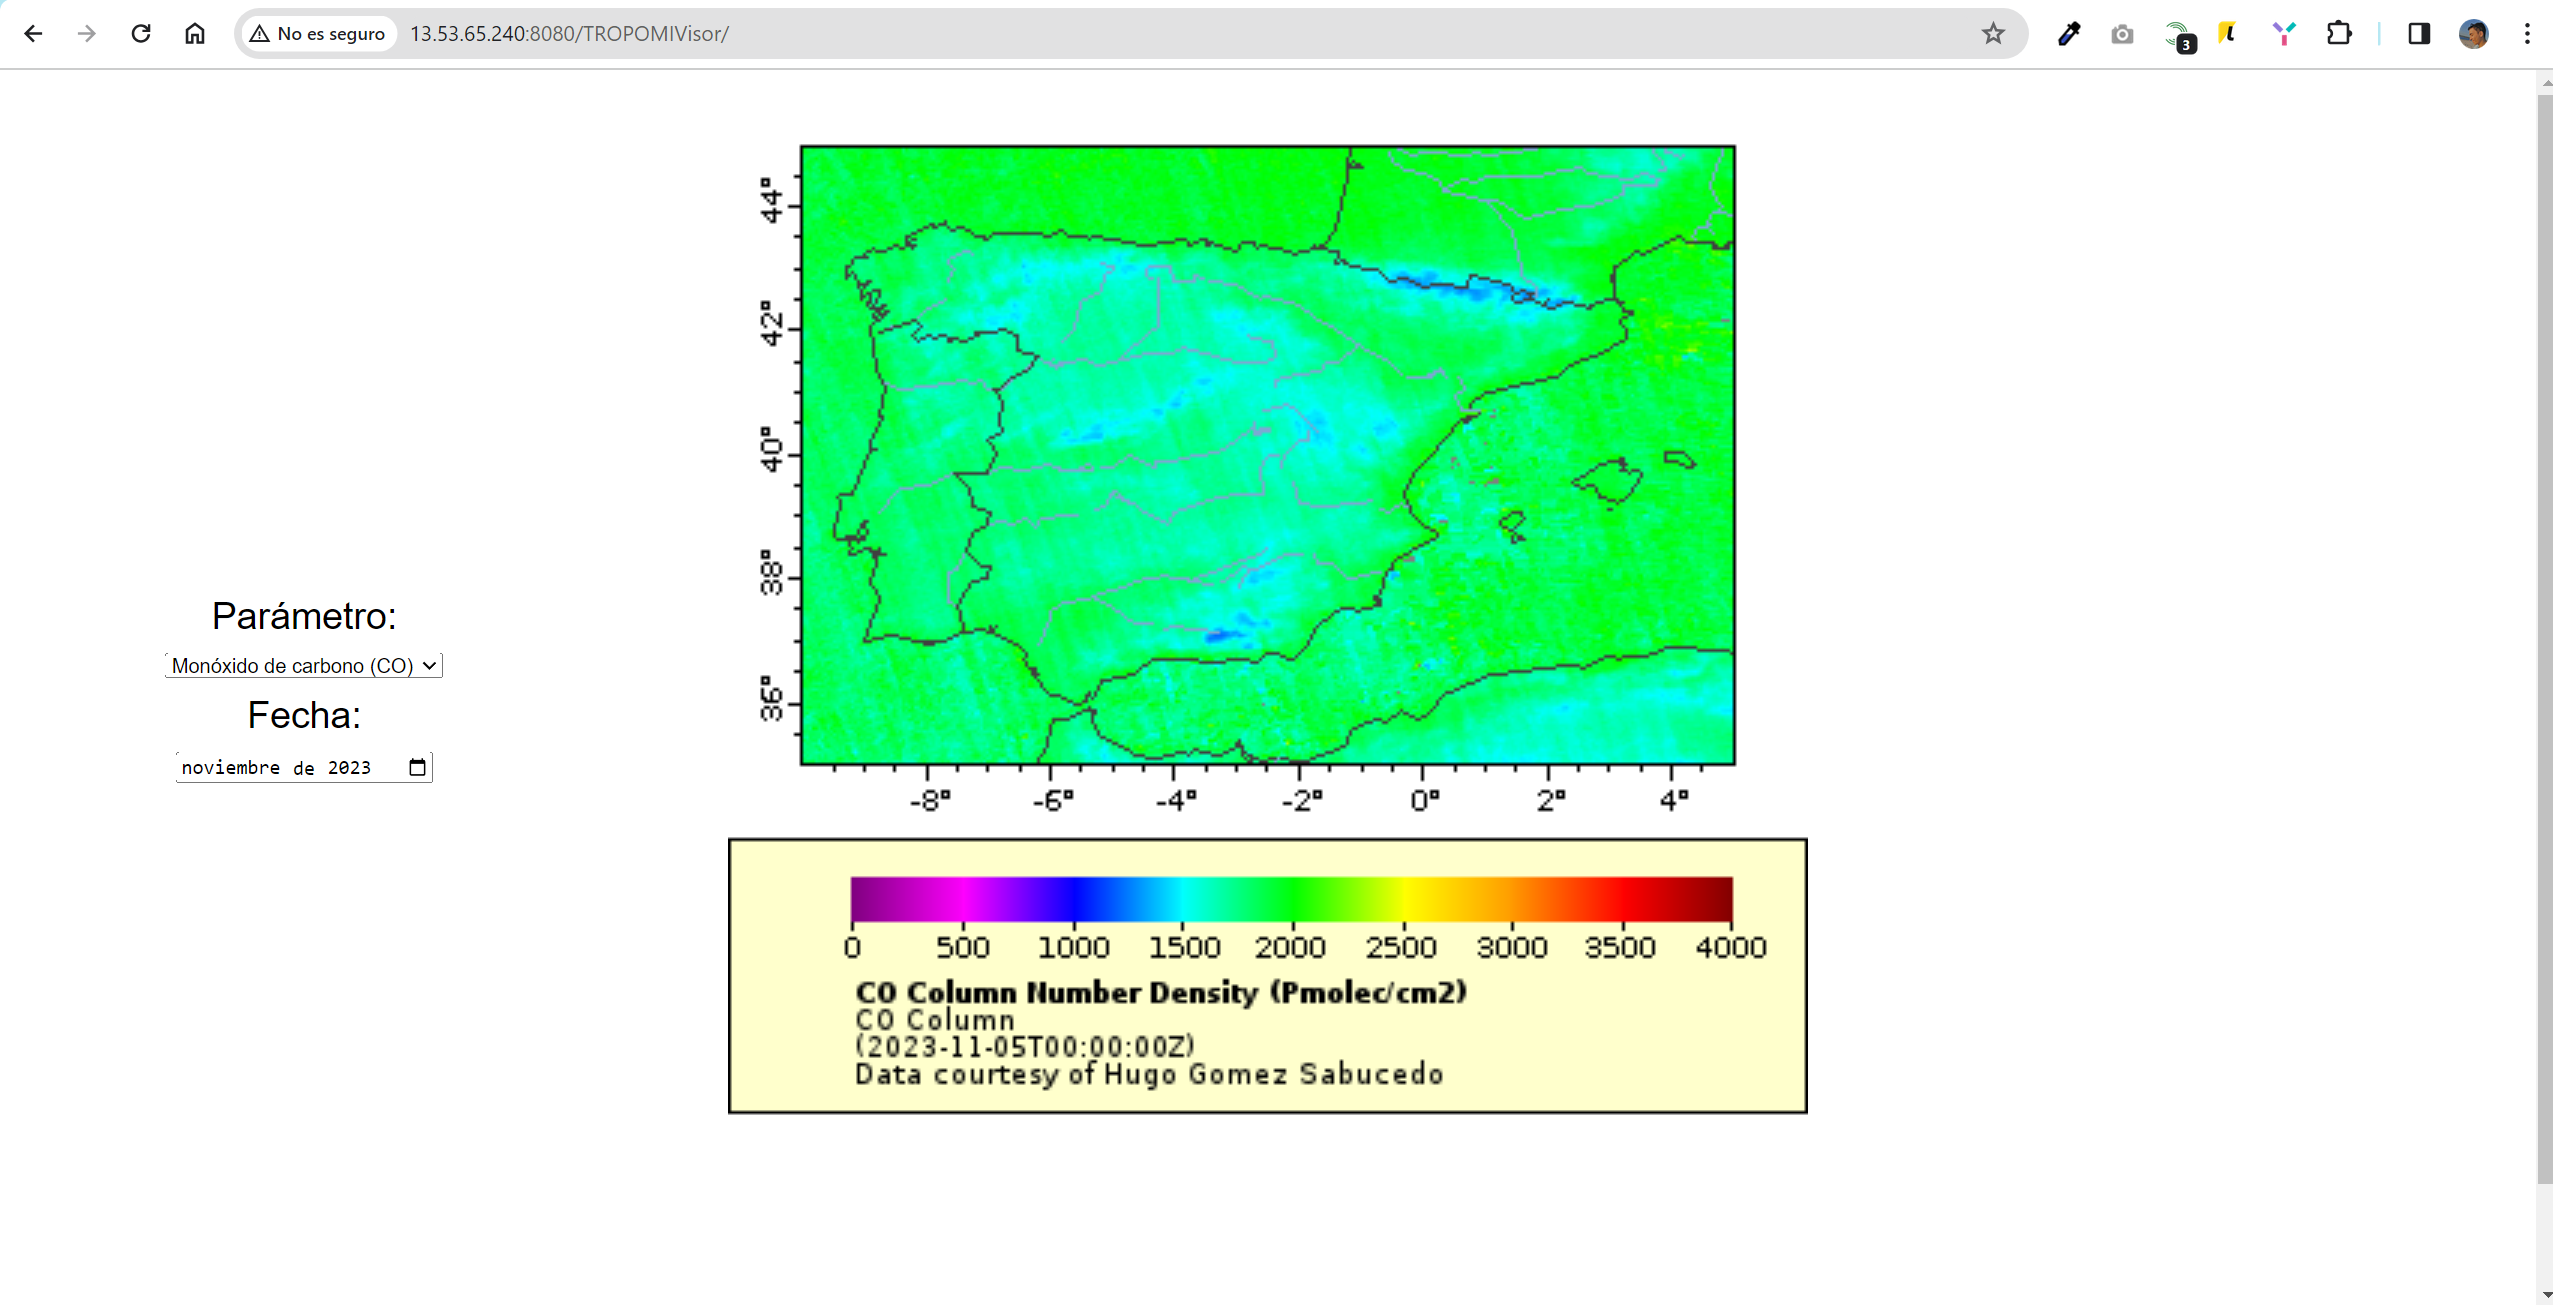
\includegraphics[width=10cm]{figuras/interfaz.png}}
    \caption{Exemplo da interface que se mostra ó acceder á aplicación.}
    \label{fig:interfaz}
\end{figure}
